\clearpage
\subsectionold{MSVC: x86 + \olly}
\myindex{\olly}

Things are even simpler here:

\begin{figure}[H]
\centering
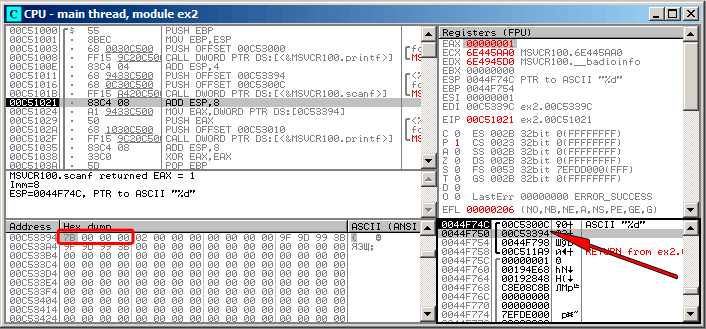
\includegraphics[scale=\FigScale]{patterns/04_scanf/2_global/ex2_olly_1.png}
\caption{\olly: after \scanf execution}
\label{fig:scanf_ex2_olly_1}
\end{figure}

The variable is located in the data segment.
After the \PUSH instruction (pushing the address of $x$) gets executed, 
the address appears in the stack window. Right-click on that row and select \q{Follow in dump}.
The variable will appear in the memory window on the left.
After we have entered 123 in the console, 
\TT{0x7B} appears in the memory window (see the highlighted screenshot regions).

But why is the first byte \TT{7B}?
Thinking logically, \TT{00 00 00 7B} should be
there.
The cause for this is referred as  \gls{endianness}, and x86 uses \IT{little-endian}.
This implies that the lowest byte is written first, and the highest written last.
Read more about it at: \myref{sec:endianness}.
Back to the example, the 32-bit value is loaded from this memory address into \EAX and passed to \printf.

The memory address of $x$ is \TT{0x00C53394}.

\clearpage
In \olly we can review the process memory map (Alt-M)
and we can see that this address is inside the \TT{.data} PE-segment of our program:

\begin{figure}[H]
\centering
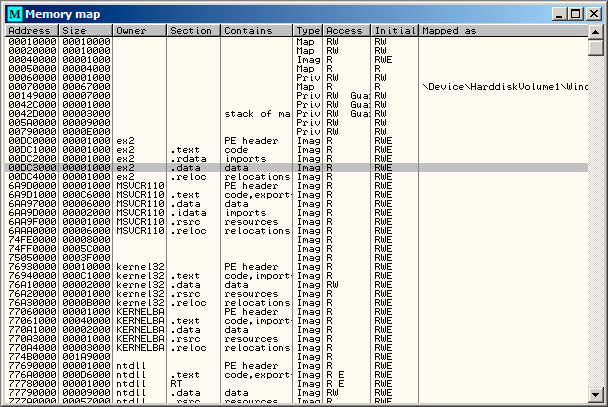
\includegraphics[scale=\FigScale]{patterns/04_scanf/2_global/ex2_olly_2.png}
\caption{\olly: process memory map}
\label{fig:scanf_ex2_olly_2}
\end{figure}

